Várias vezes, no entanto, os dados não apresentam relação linear. Nesses casos, é importante encontrar alguma técnica de linearização que transforma os dados para novos valores dependentes, mas que se relacionam de maneira linear. Algo como a relação \ref{eq:linearizacao}.

\begin{equacao} \label{eq:linearizacao}
    f(x, y) = a + b ~ g(x, y)
\end{equacao}

Dentre as técnicas mais comuns, muitas envolvem a aplicação de logaritmos para linearizar alguma relação de potência de $x$, isto é, nos casos de $y \propto x^k$, ou alguma relação exponencial, $y \propto k^x$. Para esses casos, é comum a utilização de escala logarítmica na intenção de se observar melhor os dados, em que $f(x, y) = \log(y)$ e $g(x, y) = \log(x)$.


\subsection{Gráfico Log-Log}

    \begin{figure}[htbp]
        \centering
        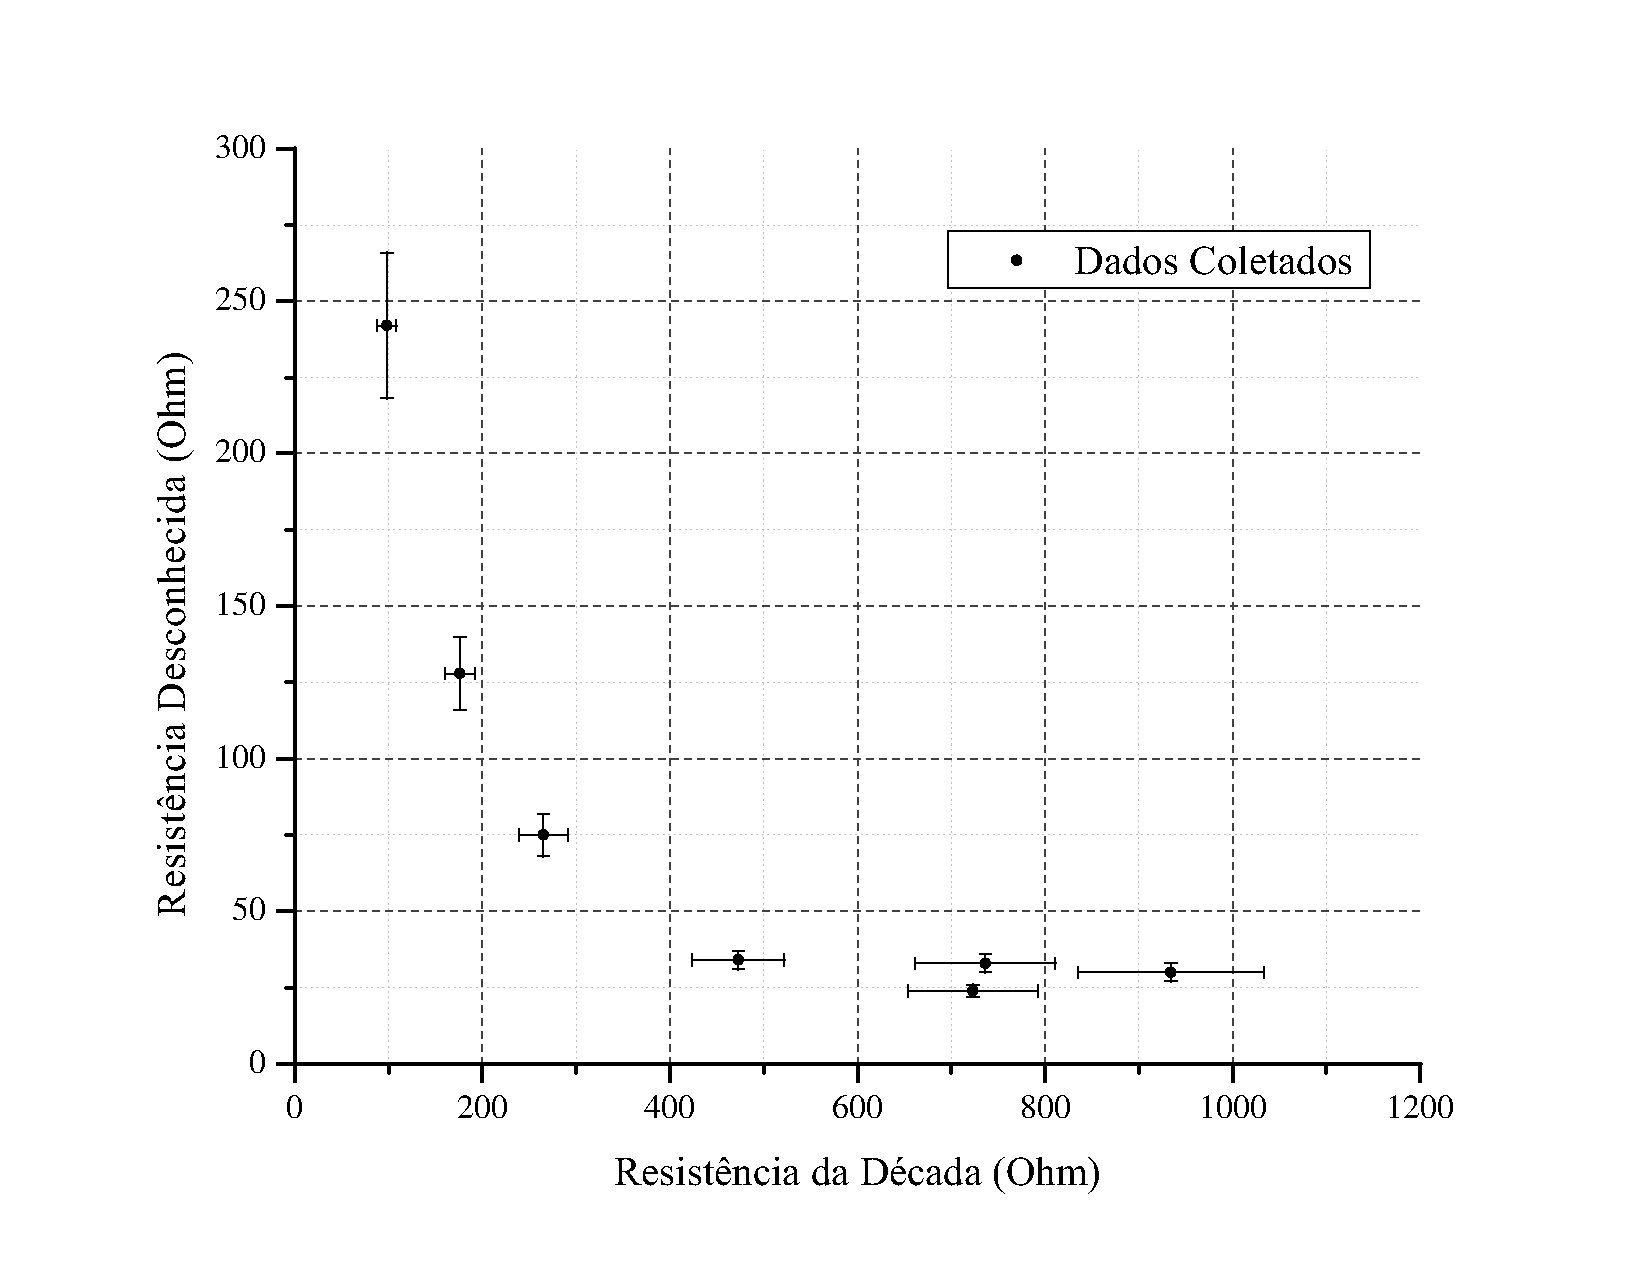
\includegraphics[width=0.6\textwidth]{escala/1dados.pdf}

        \caption{Gráfico da relação da ponte de Wheatstone (\ref{eq:wheatstone})}
        \label{fig:escala:loglog:dados}
    \end{figure}

    \begin{equacao} \label{eq:wheatstone}
        R_x = \frac{R_1 R_2}{R_d}
    \end{equacao}

    Se imaginarmos os dados do gráfico \ref{fig:escala:loglog:dados} como parte de um caso da ponte de Wheatstone dado pela equação \ref{eq:wheatstone}, sendo $R_d$ a resistência da década e $R_x$ a resistência desconhecida, podemos aplicar a seguinte técnica de linearização:

    \begin{align*}
        \log(R_x)
            &= \log\left(R_1 R_2 ~ (R_d)^{-1}\right) \\
            &= \log(R_1 R_2) + \log\left((R_d)^{-1}\right) \\
            &= \log(R_1 R_2) - \log(R_d)
    \end{align*}

    Portanto, podemos montar um gráfico \texttt{log-log} de $R_x$ por $R_d$, cujo coeficiente angular deveria resultar em $-1$.

    \begin{lembrete}
        Cuidado com o posicionamento dos dados na escala logarítmica. Normalmente quando se muda a escala, os ponto mudam de posição em suas novas representações no gráfico e apresentação dos dados pode ser prejudicada. Para atualizar essas posições, o método mais simples é permitir a mudança automática dos limites do gráfico (como na figura \ref{fig:escala:rescale}) e alterar alguma célula da tabela, servindo apenas um simples "copiar e colar" do valor que estava na célula.
    \end{lembrete}

    \begin{figure}[htbp]
        \centering
        \begin{subfigure}{0.45\textwidth}
            \centering
            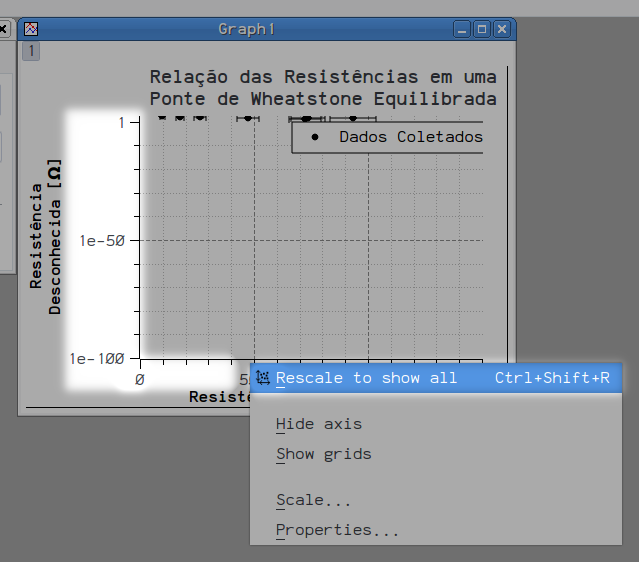
\includegraphics[width=\textwidth]{escala/2rescale.png}

            \caption{Mudança automática dos limites do gráfico}
            \label{fig:escala:rescale}
        \end{subfigure}
        ~
        \begin{subfigure}{0.45\textwidth}
            \centering
            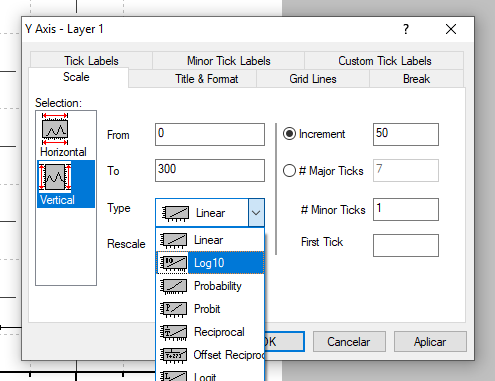
\includegraphics[width=\textwidth]{escala/3logscale.png}

            \caption{Escala logarítmica de base 10}
            \label{fig:escala:logscale}
        \end{subfigure}
        \caption{Colocando a escala logarítmica}
        \label{fig:escala:tutorial}
    \end{figure}

    \begin{figure}[htbp]
        \centering
        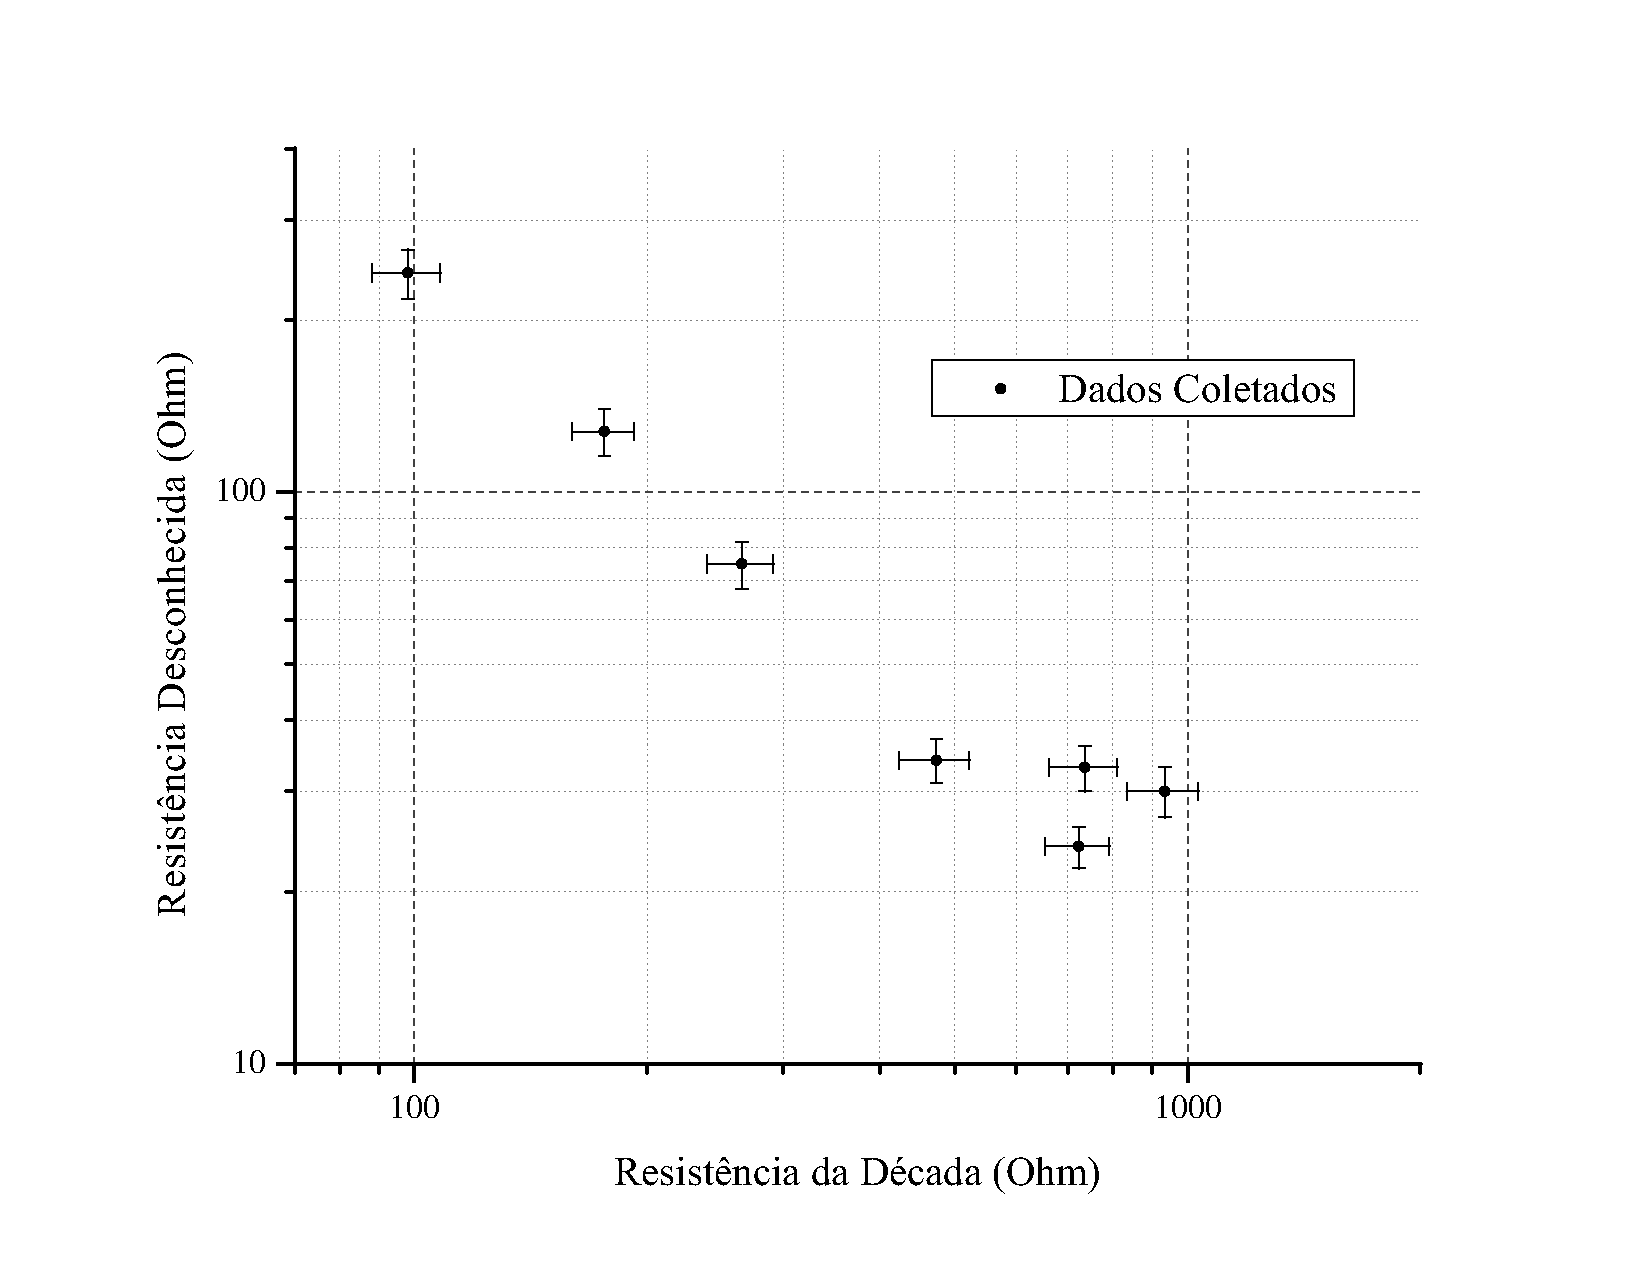
\includegraphics[width=0.8\textwidth]{escala/4loglog.pdf}

        \caption{Gráfico \texttt{log-log} dos dados da figura \ref{fig:escala:loglog:dados}}
        \label{fig:escala:loglog:resultado}
    \end{figure}


\subsection{Gráfico Semi-Log}

    \begin{figure}[htbp]
        \centering
        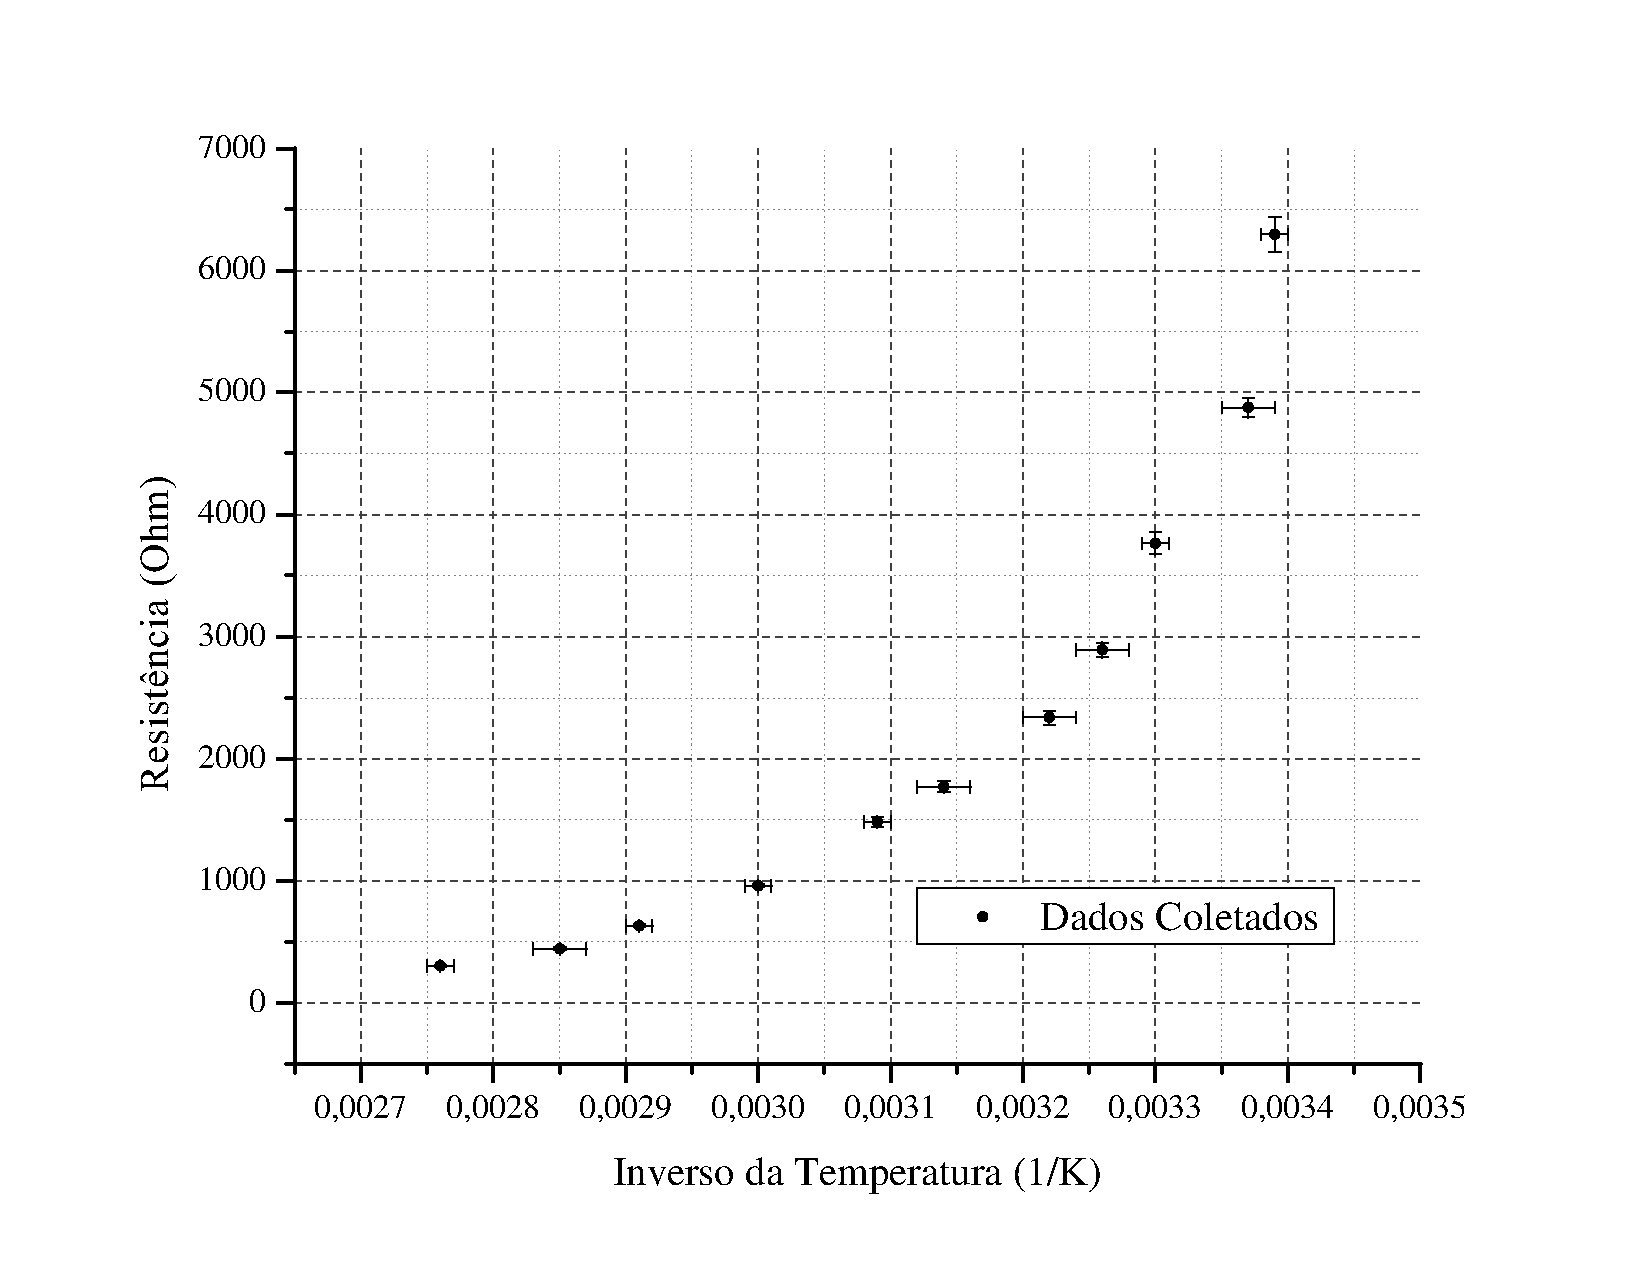
\includegraphics[width=0.6\textwidth]{escala/5dados.pdf}

        \caption{Gráfico da relação (\ref{eq:termistor}) do termistor}
        \label{fig:escala:semilog:dados}
    \end{figure}

    \begin{equacao} \label{eq:termistor}
        R = A ~ \exp\left(B ~ T^{-1}\right)
    \end{equacao}

    Agora com os dados da figura \ref{fig:escala:semilog:dados} e a relação (\ref{eq:termistor}), com $R$ como a resistência e $T^{-1}$ o inverso da temperatura, a linearização se torna:

    \begin{align*}
        \ln(R)
            &= \ln\left(A ~ \exp\left(B ~ T^{-1}\right) \right) \\
            &= \ln(A) + \ln\left(\exp\left(B ~ T^{-1}\right) \right) \\
            &= \ln(A) + B ~ T^{-1}
    \end{align*}

    Que pode ser usada em um gráfico \texttt{semi-log} de $R \times T^{-1}$, como na figura \ref{fig:escala:tutextra}.

    \begin{figure}[htbp]
        \centering
        \begin{subfigure}{0.45\textwidth}
            \centering
            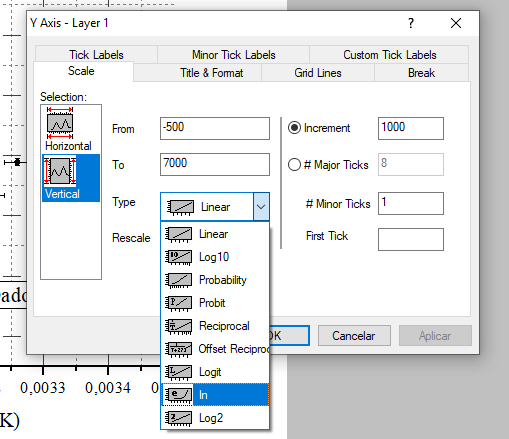
\includegraphics[width=\textwidth]{escala/6lnscale.png}

            \caption{Escala logarítmica de base $e$}
            \label{fig:escala:lnscale}
        \end{subfigure}
        ~
        \begin{subfigure}{0.45\textwidth}
            \centering
            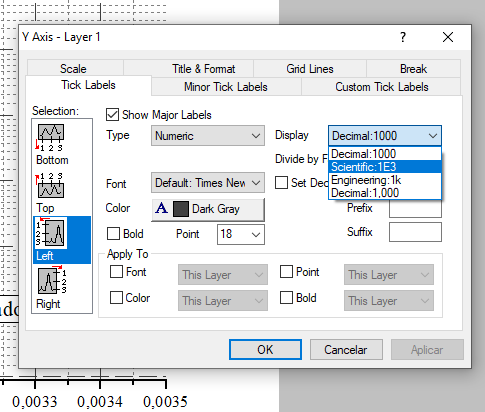
\includegraphics[width=\textwidth]{escala/7expticks.png}

            \caption{Marcadores de escala como expoentes de $e$}
            \label{fig:escala:expticks}
        \end{subfigure}
        \caption{Ajustes para a escala \texttt{ln}}
        \label{fig:escala:tutextra}
    \end{figure}

    \begin{figure}[htbp]
        \centering
        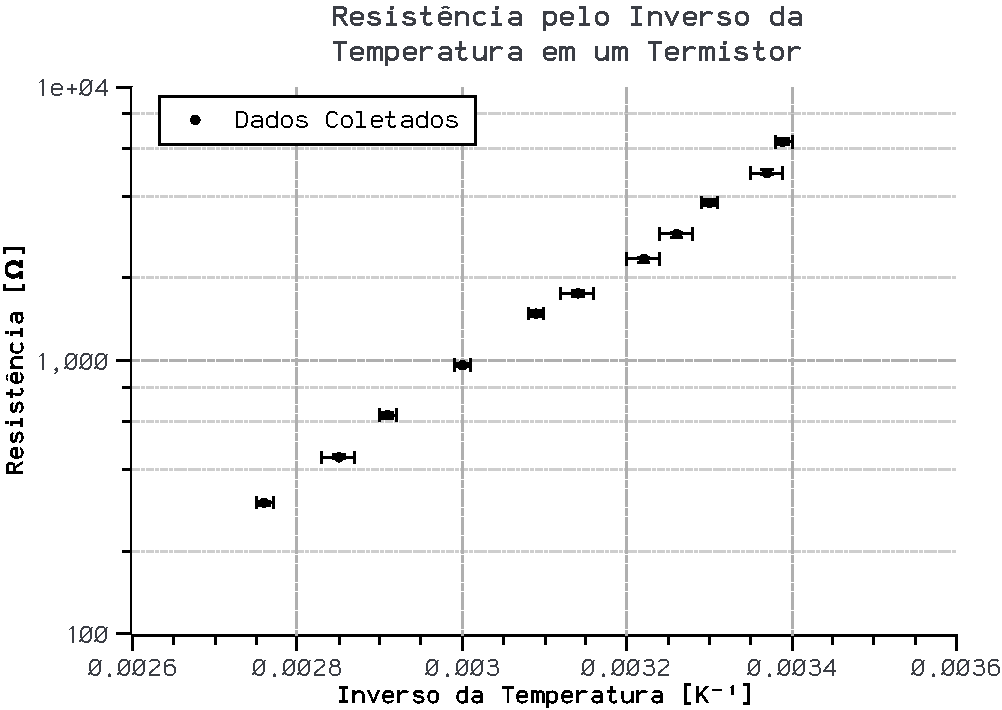
\includegraphics[width=0.8\textwidth]{escala/8semilog.pdf}

        \caption{Gráfico \texttt{semi-log} dos dados da figura \ref{fig:escala:semilog:dados}}
        \label{fig:escala:semilog:resultado}
    \end{figure}


\subsection{Regressão em Escala Logarítmica}

    A regressão de uma curva de potência ou exponencial é possível com técnicas de regressão não-linear, só que essas técnicas não cabem no escopo dessa matéria. Uma outra opção muito utilizada é encontrar uma linearização, como na equação (\ref{eq:linearizacao}), e, com a nova relação linear de $f(x, y) \times g(x, y)$, aplicar a regressão linear como da seção \nameref{sec:regres}. O único detalhe é que é preciso encontrar os valores de $f(x, y)$ e $g(x, y)$ e suas incertezas para cada par $(x, y)$ dos dados e só com esses valores pode-se encontrar os coeficientes $a$ e $b$, como foi feito na figura \ref{fig:escala:regres}.

    \begin{figure}[htbp]
        \centering
        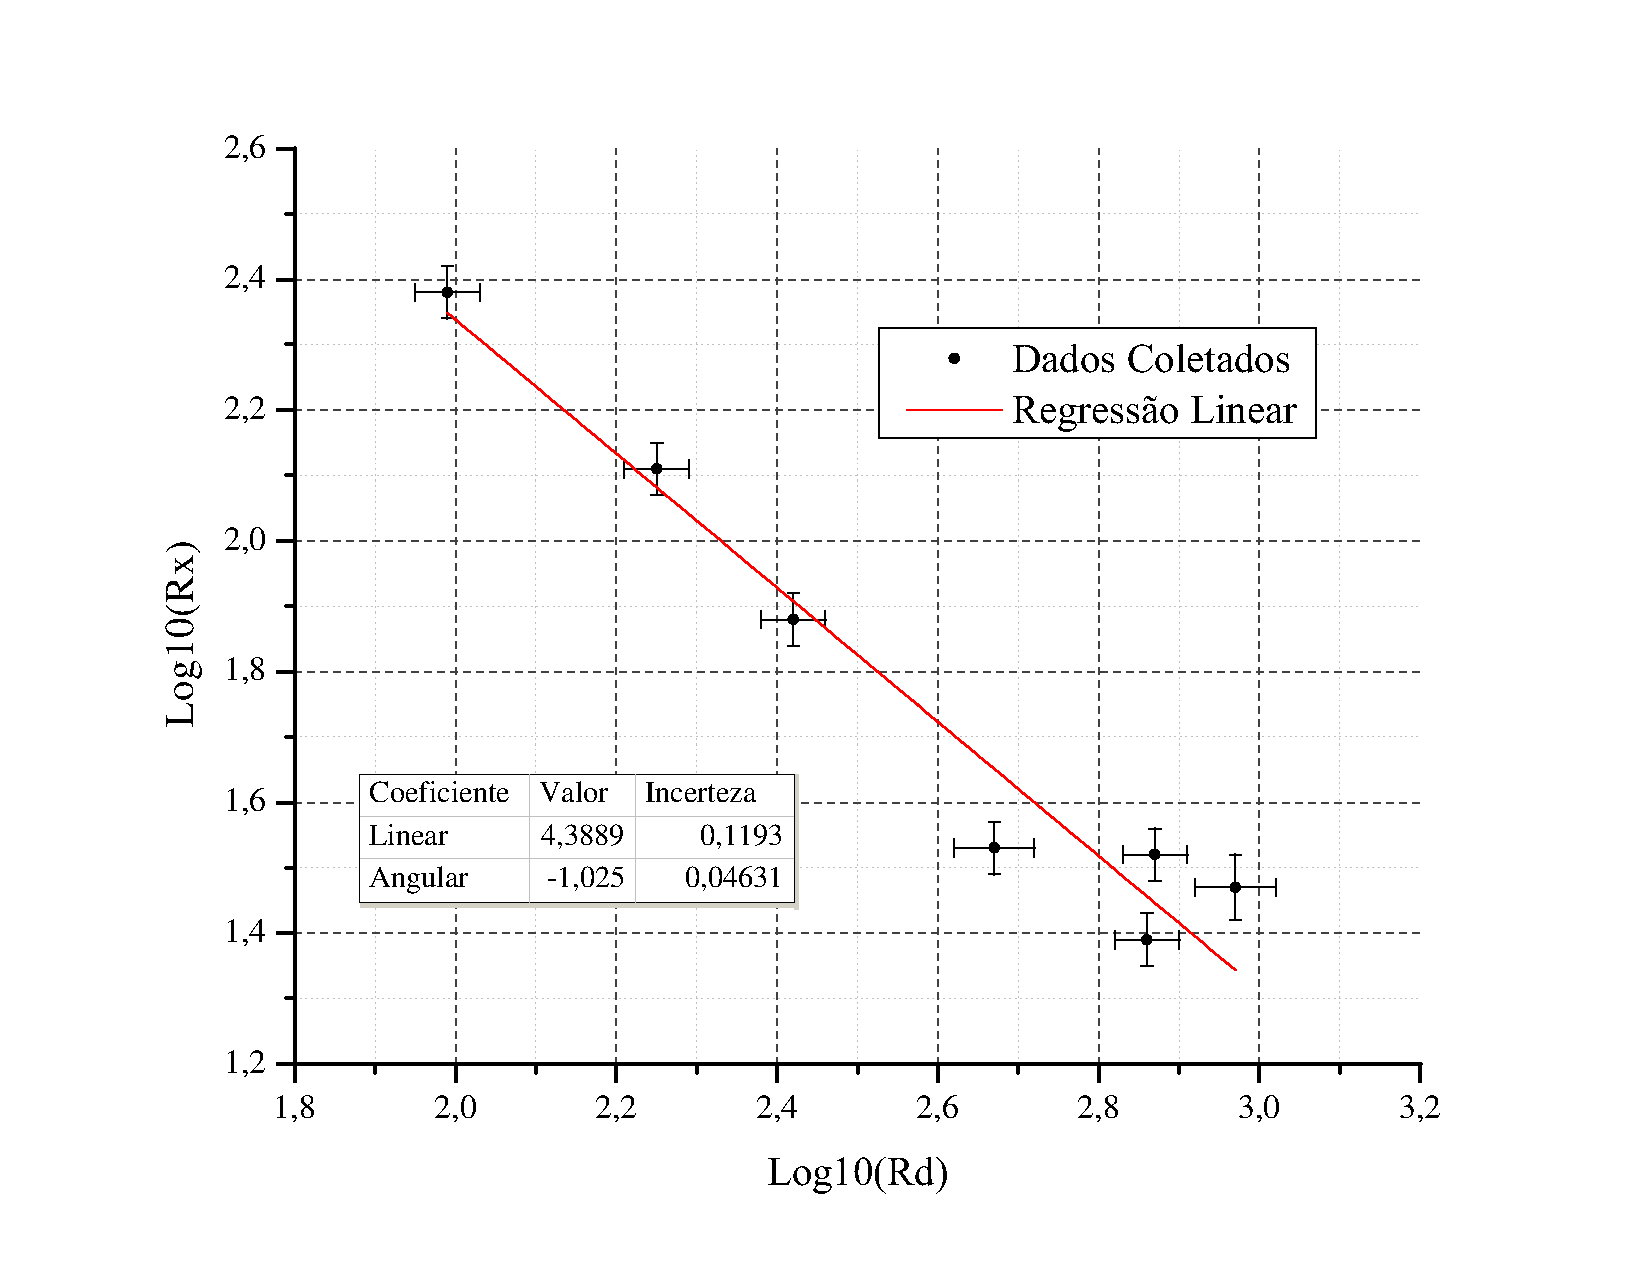
\includegraphics[width=0.8\textwidth]{escala/9logreg.pdf}

        \caption{Gráfico da regressão da relação (\ref{eq:wheatstone}). Isso seviria para mostrar que $b \approx -1$, por exemplo.}
        \label{fig:escala:regres}
    \end{figure}

    A mudança dos dados de $(x, y)$ para $(f(x, y), g(x, y))$ ajuda nos cálculos, só que normalmente causa um distanciamento do sentido físco dos dados. Então, é importante decidir qual dos gráficos utilizar ou se cabe usar os dois gráficos.
